\let\negmedspace\undefined
\let\negthickspace\undefined
%\RequirePackage{amsmath}
\documentclass[journal,12pt,twocolumn]{IEEEtran}
%
% \usepackage{setspace}
 \usepackage{gensymb}
%\doublespacing
 \usepackage{polynom}
%\singlespacing
%\usepackage{silence}
%Disable all warnings issued by latex starting with "You have..."
%\usepackage{graphicx}
\usepackage{amssymb}
%\usepackage{relsize}
\usepackage[cmex10]{amsmath}
%\usepackage{amsthm}
%\interdisplaylinepenalty=2500
%\savesymbol{iint}
%\usepackage{txfonts}
%\restoresymbol{TXF}{iint}
%\usepackage{wasysym}
\usepackage{amsthm}
%\usepackage{pifont}
%\usepackage{iithtlc}
% \usepackage{mathrsfs}
% \usepackage{txfonts}
 \usepackage{stfloats}
% \usepackage{steinmetz}
 \usepackage{bm}
% \usepackage{cite}
% \usepackage{cases}
% \usepackage{subfig}
%\usepackage{xtab}
\usepackage{longtable}
%\usepackage{multirow}
%\usepackage{algorithm}
%\usepackage{algpseudocode}
\usepackage{enumitem}
 \usepackage{mathtools}
 \usepackage{tikz}
% \usepackage{circuitikz}
% \usepackage{verbatim}
%\usepackage{tfrupee}
\usepackage[breaklinks=true]{hyperref}
%\usepackage{stmaryrd}
%\usepackage{tkz-euclide} % loads  TikZ and tkz-base
%\usetkzobj{all}
\usepackage{listings}
    \usepackage{color}                                            %%
    \usepackage{array}                                            %%
    \usepackage{longtable}                                        %%
    \usepackage{calc}                                             %%
    \usepackage{multirow}                                         %%
    \usepackage{hhline}                                           %%
    \usepackage{ifthen}                                           %%
  %optionally (for landscape tables embedded in another document): %%
    \usepackage{lscape}     
% \usepackage{multicol}
% \usepackage{chngcntr}
%\usepackage{enumerate}

%\usepackage{wasysym}
%\newcounter{MYtempeqncnt}
\DeclareMathOperator*{\Res}{Res}
\DeclareMathOperator*{\equals}{=}
%\renewcommand{\baselinestretch}{2}
\renewcommand\thesection{\arabic{section}}
\renewcommand\thesubsection{\thesection.\arabic{subsection}}
\renewcommand\thesubsubsection{\thesubsection.\arabic{subsubsection}}

\renewcommand\thesectiondis{\arabic{section}}
\renewcommand\thesubsectiondis{\thesectiondis.\arabic{subsection}}
\renewcommand\thesubsubsectiondis{\thesubsectiondis.\arabic{subsubsection}}

% correct bad hyphenation here
\hyphenation{op-tical net-works semi-conduc-tor}
\def\inputGnumericTable{}                                 %%

\lstset{
%language=C,
frame=single, 
breaklines=true,
columns=fullflexible
}
%\lstset{
%language=tex,
%frame=single, 
%breaklines=true
%}
\begin{document}

%


\newtheorem{theorem}{Theorem}[section]
\newtheorem{problem}{Problem}
\newtheorem{proposition}{Proposition}[section]
\newtheorem{lemma}{Lemma}[section]
\newtheorem{corollary}[theorem]{Corollary}
\newtheorem{example}{Example}[section]
\newtheorem{definition}[problem]{Definition}
%\newtheorem{thm}{Theorem}[section] 
%\newtheorem{defn}[thm]{Definition}
%\newtheorem{algorithm}{Algorithm}[section]
%\newtheorem{cor}{Corollary}
\newcommand{\BEQA}{\begin{eqnarray}}
\newcommand{\EEQA}{\end{eqnarray}}
\newcommand{\define}{\stackrel{\triangle}{=}}
\newcommand*\circled[1]{\tikz[baseline=(char.base)]{
    \node[shape=circle,draw,inner sep=2pt] (char) {#1};}}
\bibliographystyle{IEEEtran}
%\bibliographystyle{ieeetr}
\providecommand{\mbf}{\mathbf}
\providecommand{\pr}[1]{\ensuremath{\Pr\left(#1\right)}}
\providecommand{\qfunc}[1]{\ensuremath{Q\left(#1\right)}}
\providecommand{\sbrak}[1]{\ensuremath{{}\left[#1\right]}}
\providecommand{\lsbrak}[1]{\ensuremath{{}\left[#1\right.}}
\providecommand{\rsbrak}[1]{\ensuremath{{}\left.#1\right]}}
\providecommand{\brak}[1]{\ensuremath{\left(#1\right)}}
\providecommand{\lbrak}[1]{\ensuremath{\left(#1\right.}}
\providecommand{\rbrak}[1]{\ensuremath{\left.#1\right)}}
\providecommand{\cbrak}[1]{\ensuremath{\left\{#1\right\}}}
\providecommand{\lcbrak}[1]{\ensuremath{\left\{#1\right.}}
\providecommand{\rcbrak}[1]{\ensuremath{\left.#1\right\}}}
\theoremstyle{remark}
\newtheorem{rem}{Remark}
\newcommand{\sgn}{\mathop{\mathrm{sgn}}}
\providecommand{\abs}[1]{\left\vert#1\right\vert}
\providecommand{\res}[1]{\Res\displaylimits_{#1}} 
\providecommand{\norm}[1]{\left\lVert#1\right\rVert}
%\providecommand{\norm}[1]{\lVert#1\rVert}
\providecommand{\mtx}[1]{\mathbf{#1}}
\providecommand{\mean}[1]{E\left[ #1 \right]}
\providecommand{\fourier}{\overset{\mathcal{F}}{ \rightleftharpoons}}
%\providecommand{\hilbert}{\overset{\mathcal{H}}{ \rightleftharpoons}}
\providecommand{\system}{\overset{\mathcal{H}}{ \longleftrightarrow}}
	%\newcommand{\solution}[2]{\textbf{Solution:}{#1}}
\newcommand{\solution}{\noindent \textbf{Solution: }}
\newcommand{\cosec}{\,\text{cosec}\,}
\providecommand{\dec}[2]{\ensuremath{\overset{#1}{\underset{#2}{\gtrless}}}}
\newcommand{\myvec}[1]{\ensuremath{\begin{pmatrix}#1\end{pmatrix}}}
\newcommand{\mydet}[1]{\ensuremath{\begin{vmatrix}#1\end{vmatrix}}}
\numberwithin{equation}{section}
\numberwithin{figure}{section}
\numberwithin{table}{section}
%\numberwithin{equation}{subsection}
%\numberwithin{problem}{section}
%\numberwithin{definition}{section}
\makeatletter
\@addtoreset{figure}{problem}
\makeatother
\let\StandardTheFigure\thefigure
\let\vec\mathbf
%\renewcommand{\thefigure}{\theproblem.\arabic{figure}}
\renewcommand{\thefigure}{\theproblem}
%\setlist[enumerate,1]{before=\renewcommand\theequation{\theenumi.\arabic{equation}}
%\counterwithin{equation}{enumi}
%\renewcommand{\theequation}{\arabic{subsection}.\arabic{equation}}
\def\putbox#1#2#3{\makebox[0in][l]{\makebox[#1][l]{}\raisebox{\baselineskip}[0in][0in]{\raisebox{#2}[0in][0in]{#3}}}}
     \def\rightbox#1{\makebox[0in][r]{#1}}
     \def\centbox#1{\makebox[0in]{#1}}
     \def\topbox#1{\raisebox{-\baselineskip}[0in][0in]{#1}}
     \def\midbox#1{\raisebox{-0.5\baselineskip}[0in][0in]{#1}}
\vspace{3cm}
\title{Probability and random variables assignment}
\author{Maharshi Kadeval}

\maketitle

\newpage

\bigskip

\numberwithin{equation}{section}
\numberwithin{figure}{section}
\numberwithin{table}{section}
\section{Q8 c)}
\begin{enumerate}[label=\thesection.\arabic*.,ref=\thesection.\theenumi]
\numberwithin{equation}{enumi}
\numberwithin{figure}{enumi}
\numberwithin{table}{enumi}
\item Using ruler and compass only, construct a $\bigtriangleup$ABC such that BC = 5 cm
and AB = 6.5 cm and $\angle$ABC = 120°\\
(i) Construct a circum-circle of $\bigtriangleup$ABC\\
(ii) Construct a cyclic quadrilateral ABCD, such that D is equidistant from AB and BC.\\

\solution The parameters for constructing the figure are given in the table below:

\begin{table}[h]
\centering
\caption{}
\begin{tabular}{|c|c|p{3.5cm}|}
\hline
\textbf{Symbol} & \textbf{Value} & \textbf{Description}\\
\hline
$a$ & $5$ & $BC$\\
\hline
$c$ & $6.5$ & $AB$\\
\hline
$\alpha$ & $\cot^{-1} \frac{11*\sqrt{3}}{13}$ & $\angle ACB$\\
\hline
$\theta$ & $\frac{\pi}{3}$ & $\pi - \angle ABC$\\
\hline
$l$ & $\frac{6.5*\sqrt{3}}{2*\sin \alpha}$ & $AD$\\
\hline
$A$ & $\myvec{0 \\ 0}$ & origin\\
\hline
$B$ & $\myvec{c \\ 0}$ & point of triangle\\
\hline
$C$ & $\myvec{c+a*\cos \theta \\ a*\sin \theta}$ & point of triangle\\
\hline
$E$ & $\myvec{c/2 \\ \brak{c/2}*\cot \alpha}$ & centre of circumcircle of $\bigtriangleup$ABC.\\
\hline
$r$ & $\frac{c}{2\sin \alpha}$ & radius of circumcircle of $\bigtriangleup$ABC.\\
\hline
$D$ & $l*\myvec{\cos \brak{2\theta - \alpha} \\ \sin \brak{2\theta - \alpha}}$ & intersection point of angle bisector of AB and BC and circumcircle\\
\hline
\end{tabular} 	
\end{table}

\textbf{Deriving the coordinates of C,D,E and the radius r:}\\

X-coordinate of any point is the perpendicular distance\brak{algebraic} of point from Y-axis\\
Y-coordinate of any point is the perpendicular distance\brak{algebraic} of point from X-axis\\

Let foot of perpendicular from C to X-axis be F and C = \myvec{X_c \\ Y_c}\\
$X_c=AB+BF$ and $Y_c = CF$\\
from trigonometry $BF = BC\cos \theta = a*\cos \theta$ and $CF = BC\sin \theta = a*\sin \theta$ \\
$X_c = c + a*\cos \theta$ and $Y_c = a*\sin \theta$ \\ 
$\therefore C = \myvec{c + a\cos \theta \\ a\sin \theta} $\\
Using Sine rule in $\bigtriangleup$ABC, we find $\alpha$\\
Let E = \myvec{X_E \\ Y_E} and foot of perpendicular from E to X-axis be G.
Using the fact that angle subtended by a chord at any point of the circle is half of that subtended at the centre,
$\angle AEB = 2\alpha$ \\
Since E is centre of circumcircle, EA = EB and hence $\bigtriangleup$AEB is isoceles by which we conclude that $\angle AEG = \angle BEG = \alpha$
Using trigonometry in $\bigtriangleup$AEG
$X_E=c/2$, $\cot \alpha = \frac{Y_E}{X_E}$ and $\cosec \alpha = \frac{r}{X_E}$, \\
$Y_E=\brak{c/2}\cot \alpha $\\ 
$\therefore E = \myvec{c/2 \\ \brak{c/2}\cot \alpha} $ and $r=\frac{c}{2\sin \alpha} $\\
$l$ is found by applying sine rule in $\bigtriangleup$ADB\\
Let D = \myvec{X_D \\ Y_D} and foot of perpendicular from D to X-axis be H,
and given that AD=l\\
From geometry $\angle DAB = 2\theta-\alpha$,
Using trigonometry in $\bigtriangleup$ADH, 
$AH=X_D=l\cos \brak{2\theta-\alpha}$and $DH=Y_D=l\sin \brak{2\theta-\alpha}$
$\therefore D = l*\myvec{\cos \brak{2\theta-\alpha} \\ \sin \brak{2\theta-\alpha}} $\\
\\
\textbf{Table for Output parameters:}
\begin{table}[h]
\centering
\caption{}
\begin{tabular}{|c|c|p{3.5cm}|}
\hline
\textbf{Symbol} & \textbf{Value} & \textbf{Description}\\
\hline
$\alpha$ & $\cot^{-1} \frac{11*\sqrt{3}}{13}$ & $\angle ACB$\\
\hline
$l$ & $\frac{6.5*\sqrt{3}}{2*\sin \alpha}$ & $AD$\\
\hline
$C$ & $\myvec{c+a*\cos \theta \\ a*\sin \theta}$ & point of triangle\\
\hline
$E$ & $\myvec{c/2 \\ \brak{c/2}*\cot \alpha}$ & centre of circumcircle of $\bigtriangleup$ABC.\\
\hline
$r$ & $\frac{c}{2\sin \alpha}$ & radius of circumcircle of $\bigtriangleup$ABC.\\
\hline
$D$ & $l*\myvec{\cos \brak{2\theta - \alpha} \\ \sin \brak{2\theta - \alpha}}$ & intersection point of angle bisector of AB and BC and circumcircle\\
\hline
 \end{tabular} 	
\end{table}

\textbf{Steps of construction}:\\

1. The point A is taken as origin and a line segment AB = 6.5 cm is drawn along positive x-axis.\\

2. Draw a line segment emerging from B at $\angle$120° in anticlockwise direction from BA of length 5 cm.\\

3. Name the other endpoint of the line segment as C.\\

4. Join AC. This completes the $\bigtriangleup$ABC.\\

5. Now take the perpendicular bisector of any two sides, mark their point of intersection as E(centre of circumcircle).\\

6. Taking E as centre and EA=EB=EC as radius draw a circle(circumcircle).\\

7. Take internal angle bisector of AB and BC, let its point of intersection with the circumcircle be D.\\

8. Join AD and CD.\\


(i)\ref{fig1} \\
center of the circumcircle is the point of intersection of the perpendicular bisectors of AB and BC.
\begin{figure}[h!]
\centering
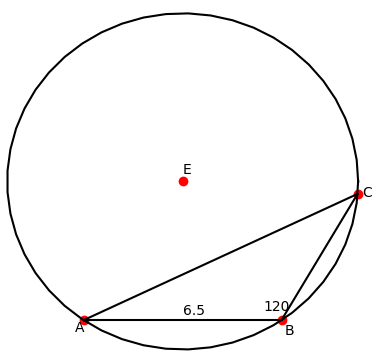
\includegraphics[width = \columnwidth]{fig1.png}
\caption{}
\label{fig1}
\end{figure}

(ii)\ref{fig2} \\
the point D of the cyclic quadrilateral ABCD is the point of intersection of the angle 
bisectors of AB and BC and the circumcircle.
\begin{figure}[t!]
\centering
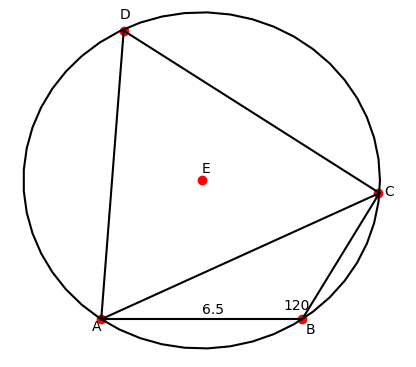
\includegraphics[width = \columnwidth]{fig2.png}\\
\caption{}
\label{fig2}
\end{figure}
\\

\end{enumerate}

\end{document}